% Options for packages loaded elsewhere
\PassOptionsToPackage{unicode}{hyperref}
\PassOptionsToPackage{hyphens}{url}
%
\documentclass[
  12pt,
]{article}
\usepackage{amsmath,amssymb}
\usepackage{lmodern}
\usepackage{iftex}
\ifPDFTeX
  \usepackage[T1]{fontenc}
  \usepackage[utf8]{inputenc}
  \usepackage{textcomp} % provide euro and other symbols
\else % if luatex or xetex
  \usepackage{unicode-math}
  \defaultfontfeatures{Scale=MatchLowercase}
  \defaultfontfeatures[\rmfamily]{Ligatures=TeX,Scale=1}
\fi
% Use upquote if available, for straight quotes in verbatim environments
\IfFileExists{upquote.sty}{\usepackage{upquote}}{}
\IfFileExists{microtype.sty}{% use microtype if available
  \usepackage[]{microtype}
  \UseMicrotypeSet[protrusion]{basicmath} % disable protrusion for tt fonts
}{}
\makeatletter
\@ifundefined{KOMAClassName}{% if non-KOMA class
  \IfFileExists{parskip.sty}{%
    \usepackage{parskip}
  }{% else
    \setlength{\parindent}{0pt}
    \setlength{\parskip}{6pt plus 2pt minus 1pt}}
}{% if KOMA class
  \KOMAoptions{parskip=half}}
\makeatother
\usepackage{xcolor}
\usepackage[margin=1in]{geometry}
\usepackage{longtable,booktabs,array}
\usepackage{calc} % for calculating minipage widths
% Correct order of tables after \paragraph or \subparagraph
\usepackage{etoolbox}
\makeatletter
\patchcmd\longtable{\par}{\if@noskipsec\mbox{}\fi\par}{}{}
\makeatother
% Allow footnotes in longtable head/foot
\IfFileExists{footnotehyper.sty}{\usepackage{footnotehyper}}{\usepackage{footnote}}
\makesavenoteenv{longtable}
\usepackage{graphicx}
\makeatletter
\def\maxwidth{\ifdim\Gin@nat@width>\linewidth\linewidth\else\Gin@nat@width\fi}
\def\maxheight{\ifdim\Gin@nat@height>\textheight\textheight\else\Gin@nat@height\fi}
\makeatother
% Scale images if necessary, so that they will not overflow the page
% margins by default, and it is still possible to overwrite the defaults
% using explicit options in \includegraphics[width, height, ...]{}
\setkeys{Gin}{width=\maxwidth,height=\maxheight,keepaspectratio}
% Set default figure placement to htbp
\makeatletter
\def\fps@figure{htbp}
\makeatother
\setlength{\emergencystretch}{3em} % prevent overfull lines
\providecommand{\tightlist}{%
  \setlength{\itemsep}{0pt}\setlength{\parskip}{0pt}}
\setcounter{secnumdepth}{-\maxdimen} % remove section numbering
\usepackage{natbib}
\bibliographystyle{abbrvnat}
\setcitestyle{authoryear, open={((},close={)}}
\ifLuaTeX
  \usepackage{selnolig}  % disable illegal ligatures
\fi
\IfFileExists{bookmark.sty}{\usepackage{bookmark}}{\usepackage{hyperref}}
\IfFileExists{xurl.sty}{\usepackage{xurl}}{} % add URL line breaks if available
\urlstyle{same} % disable monospaced font for URLs
\hypersetup{
  pdftitle={Relationship between Lifestyle Risk Factors and Development of Prediabetes or Diabetes, based on BRFSS 2015 Questionnaire},
  pdfauthor={Tianyang Jiang, Changhao Jiang, Liuye Huang},
  hidelinks,
  pdfcreator={LaTeX via pandoc}}

\title{Relationship between Lifestyle Risk Factors and Development of
Prediabetes or Diabetes, based on BRFSS 2015 Questionnaire}
\author{Tianyang Jiang, Changhao Jiang, Liuye Huang}
\date{June 07, 2023}

\begin{document}
\maketitle
\begin{abstract}
This project examines the link between lifestyle factors and the risk of
prediabetes or diabetes. Using a cross-sectional design and data from
the 2015 BRFSS questionnaire, we calculate a lifestyle combination score
with random forest and construct a DAG using the PC algorithm. We
analyze the distribution of demographic, lifestyle, and medical
characteristics among participants. Regression Adjustment helps us
determine the average treatment effect, while R-learner detects
heterogeneous treatment effects in subgroups (age, income, gender). Our
findings suggest that a healthier lifestyle is associated with a lower
risk of prediabetes or diabetes. However, it's important to note the
limitations of inferring causality in cross-sectional studies.
Identifying vulnerable groups can guide prioritized preventive measures,
with particular attention to low-income individuals, women, and
middle-aged to elderly individuals.
\end{abstract}

\textbf{Keywords:} Diabetes, Lifestyle intervention, Causal inference,
R-learner, PC algorithm, Regression adjustment

\hypertarget{background}{%
\subsection{Background}\label{background}}

With a staggering 476.0 million prevalent cases, 1.37 million deaths,
and 67.9 million disability-adjusted life-years (DALYs) recorded in
2017, diabetes has emerged as a pressing global public health concern. A
significant portion of the burden associated with diabetes is believed
to be attributable to modifiable lifestyle risk factors, such as diet,
smoking, drinking, and physical activity, as suggested by Lin et
al.~(2021). Therefore, the purpose of this research is to examine the
connection between these modifiable lifestyle risk factors and the
likelihood of developing prediabetes or diabetes among adults in the
United States.

Given the aforementioned background, we have formulated the following
research questions:

\begin{enumerate}
\def\labelenumi{\arabic{enumi}.}
\item
  What is the nature of the relationship between lifestyle factors and
  the risk of developing prediabetes or diabetes?
\item
  Does this relationship persist even after accounting for covariates?
\item
  What are the varying effects of lifestyle factors among subgroups
  characterized by different age, gender, and income levels?
\end{enumerate}

By addressing these research questions, we aim to enhance our
understanding of the complex interplay between lifestyle factors and the
risk of prediabetes or diabetes, ultimately informing targeted
interventions and preventive measures in diverse populations.

\hypertarget{data-preparation}{%
\subsection{Data Preparation}\label{data-preparation}}

\hypertarget{data-description}{%
\subsubsection{Data Description}\label{data-description}}

Dataset for this study was collected from the The Behavioral Risk Factor
Surveillance System (BRFSS) questionnaire in 2015. BRFSS is a nationwide
telephone survey system held by the U.S. Center for Disease Control and
Prevention (CDC). It collects data on health-related risk behaviors,
chronic health conditions, and preventive services usage among the U.S.
residents. This system was initiated in 1984 and updated annually, with
more than 400,000 adults being interviewed each year.

The 2015 questionnaire contains three parts, including the core
component, optional modules, and state-added questions. The core
component consisted of information on demographic characteristics and
current health behaviors. The optional modules consisted of topics of
health status and behaviors that were not covered in the core set, such
as diabetes, immunization, and multiple cancer screening (U.S. CDC).

\hypertarget{find-scores-with-random-forest}{%
\subsubsection{Find Scores with Random
Forest}\label{find-scores-with-random-forest}}

A lifestyle combination score of behavioral factors was constructed
using the information of fruits and vegetables consumption, heavy
drinking, smoking, and physical activity. It measures the overall
healthiness of an individual's lifestyle. This score can be computed by
assigning weights to each variable based on their relative importance
and then combining the weighted scores. We use the importance function
in random forest to compute the importance of the predictor variables in
a random forest model. The importance measure is based on the decrease
in the node impurity when the variable is used for splitting in the
random forest. Then we use the scaled value of the importance to
represent the weight. Suppose the importance of each variable is
\(m_1, m_2, m_3, m_4\) and \(m_5\) respectively, then the scaled value
is \(w_i=\frac{m_i}{m_1+m_2+m_3+m_4+m_5}\), where \(i=1,2,3,4,5\). Based
on the results of the literature review, we find that smoking(\(v_1\))
and heavy drinking(\(v_2\)) will cause diabetes, while more physical
exercises(\(v_3\)), fruits(\(v_4\)) and vegetables consumption(\(v_5\))
will reduce the risk of getting diabetes. Thus the combination score is
\(Score=-w_1v_1-w_2v_2+w_3v_3+w_4v_4+w_5v_5\). We then convert the
continuous variable score into a binary variable. This is achieved
through grouping by means of the average. Scores that exceed the mean
are set to 1, representing a good lifestyle. Those that fall below the
mean are assigned 0, indicating a poor lifestyle.

\begin{longtable}[]{@{}lc@{}}
\caption{Scoring Weights for Each Covariate}\tabularnewline
\toprule()
& Weighting \\
\midrule()
\endfirsthead
\toprule()
& Weighting \\
\midrule()
\endhead
HvyAlcoholConsump & 81.3077 \\
Smoker & 63.2298 \\
PhysActivity & 220.4939 \\
Fruits & 23.4497 \\
Veggies & 46.8822 \\
\bottomrule()
\end{longtable}

\hypertarget{methods}{%
\subsection{Methods}\label{methods}}

\hypertarget{build-dag-with-pc-algorithm-and-literature-review}{%
\subsubsection{Build DAG with PC Algorithm and Literature
Review}\label{build-dag-with-pc-algorithm-and-literature-review}}

We initially employ the PC algorithm to determine the relationships
between the variables. Prior to running the PC algorithm, we assume that
all variables are discrete (as indicated by the data description) and
observed. We also assume that the graph is acyclic and adhere to the
faithfulness and Markov assumptions. The PC algorithm proceeds as
follows (Spirtes et al., 2001): starting with a complete graph, we
remove edges between variables \(X\) and \(Y\) if \(X\) and \(Y\) are
conditionally independent given \(Z\) for some (potentially empty)
conditioning set. We begin with an empty conditioning set and gradually
increase its size. Following these steps, we obtain the skeleton of the
graph. Subsequently, we identify immoralities in the graph, whereby if
variable \(W\) is not in the conditioning set that renders \(X\) and
\(Y\) conditionally independent, the configuration \(X-W-Y\) forms an
immorality. Then we used the fact that we found all immoralities to
orient more edges.

However, we encountered issues with the graph when solely relying on the
PC algorithm. For instance, it suggests a direct impact of stroke on
income, which is highly implausible. Additionally, we need to determine
the directionality of edges based on more reliable sources.

In addition to considering the exposure variables, it is crucial to
account for other factors associated with diabetes, such as covariates,
precision variables, and confounding variables. According to Bird et
al.~(2015), Nanayakkara et al.~(2021), and Lin et al.~(2021), certain
covariates like high blood pressure, stroke, heart disease, and high
cholesterol are linked to diabetes, while others like BMI directly
affect diabetes. Therefore, a comprehensive assessment and incorporation
of these variables is essential when studying diabetes.

From a more reasonable perspective, it is expected that high blood
pressure and diabetes, as well as high cholesterol and diabetes, often
coexist and influence each other (Schofield et al., 2016 \(\&\) Peter et
al., 2018). Nevertheless, in this analysis, we assume that high
cholesterol and high blood pressure impact diabetes for convenience.

Furthermore, confounding variables such as age, gender, and income, as
identified by Bird et al.~(2015), can influence the relationship between
specific exposure variables, covariates, and outcome variables in
diabetes research.

To enhance the completeness and practicality of the directed acyclic
graph (DAG), we also incorporate potentially unmeasured confounding
variables, such as air pollution, and potential precision variables,
such as genetics, to get the final DAG (Appendix). As highlighted by Ali
(2013), while individuals may experience similar environmental
exposures, some people are more susceptible to developing diabetes due
to genetic factors. Genetics, therefore, is considered a precision
variable that exclusively relates to diabetes without affecting other
variables.

\hypertarget{logistic-regression-with-adjustment}{%
\subsubsection{Logistic Regression with
Adjustment}\label{logistic-regression-with-adjustment}}

We consider the variable diabetes as the outcome variable, denoted as
\(Y\), and the variable score as the treatment variable, denoted as
\(X\). Our objective is to estimate the average causal effect of the
score on diabetes, which can be expressed as \(E[Y(X=1)] - E[Y(X=0)]\).

Before estimating the causal effect, it is essential to examine the
association between diabetes and scores. In this case, diabetes takes
the value 1 if a person has diabetes and 0 if a person does not have
diabetes. Additionally, we assume a linear relationship between the
log-odds of diabetes and scores. Hence, it is reasonable to employ a
simple logistic model to capture their relationship.

We consider the following model:
\(\text{log}(\frac{p}{1-p}) = \beta_0 + \beta_1 X\), where \(p\)
represents the probability of an individual having diabetes,
\(\frac{p}{1-p}\) represents the odds, and \(\text{log}(\frac{p}{1-p})\)
represents the log-odds. In this model, \(X\) corresponds to the score,
and \(\beta\) represents the corresponding coefficients.

Based on the Directed Acyclic Graph (DAG) shown in Graph 1, we observe
three confounding paths. These paths indicate that confounding
variables, namely age, gender, and income, simultaneously connect
diabetes and scores. Consequently, estimating the effect of the score
without accounting for these confounding variables would introduce bias.
Therefore, it is necessary to determine whether controlling for these
confounders would yield better estimates of the parameter of interest.

Using the adjustment criterion proposed by Shpitser et al.~(2012), we
conclude that adjusting for the three variables (denoted as
\(Z=\{Z_1, Z_2, Z_3\}\), where \(Z_1\) represents age, \(Z_2\)
represents income, and \(Z_3\) represents gender) is sufficient. This
adjustment blocks all spurious paths from scores to diabetes and
addresses confounding for the three variables. Moreover, it also blocks
the confounding path for the variable education. Importantly, this
adjustment does not block any of the causal paths from scores to
diabetes and does not open any spurious paths. Consequently, we can
utilize the non-parametric identification result from the observational
distribution, which states that \(E[Y(X=x)] = E[E[Y|X=x,Z]]\). Notably,
when \(Z\) satisfies the adjustment criterion, the conditional
ignorability assumption holds, i.e., \(Y_x \perp\!\!\!\perp X |Z\). This
assumption aids in recovering the causal effect and improving the
accuracy of the estimation, as highlighted by Cinelli et al.~(2022).

Since we assume a linear relationship between the log-odds of diabetes
and scores, age, income, and gender, which aligns with the
aforementioned model, the logistic regression for confounding adjustment
can be written as
\(\text{log}(\frac{p}{1-p}) = \beta_0 + \beta_1 X + \gamma_1 Z_1 + \gamma_2 Z_2 + \gamma_3 Z_3\),
where \(\gamma\) represents the corresponding coefficients.
Consequently, the average causal effect corresponds to the regression
coefficient \(\beta_1\) (Cinelli et al., 2022).

\hypertarget{identity-heterogeneous-effects-with-r-learner}{%
\subsubsection{Identity Heterogeneous Effects with
R-learner}\label{identity-heterogeneous-effects-with-r-learner}}

In this section, we investigate the heterogeneous effects of lifestyle
factors on subgroups defined by age, sex, and income using the R-learner
(Nie and Wager, 2017). This approach utilizes machine learning to
estimate treatment effects in observational studies.

The R-learner is used to estimate the Conditional Average Treatment
Effect (CATE),
\(\tau^*(z_1,z_2,z_3) = E(Y(1)-Y(0) \mid Z_1=z_1,Z_2 = z_2,Z_3 = z_3)\),
with \(Z_1\), \(Z_2\), and \(Z_3\) denoting individual features (age,
income, and gender) and \(Y_i\) is the observed outcome.

Using the \(\texttt{rlasso}\) method in \(\texttt{rlearner}\), we input
age, gender, and income as features, and a categorical score as the
treatment variable, with diabetes presence indicating observed response.
The algorithm of R-learner also includes cross-validation, we set it
with ten folds. Finally, we visualize CATE across income, gender, and
age groups.

In the visualization of CATE across different income groups, we observe
a correlation between higher income and a larger average treatment
effect within the same income bracket. This trend is particularly
pronounced among individuals earning over \$50,000 annually, where the
mean effect significantly surpasses that of other groups.

When comparing CATE across genders, it is noteworthy that the average
treatment effect for females is lower than that for males.

The CATE across age groups shows a distinct decline as age increases.
For individuals younger than 24, there is little discernible difference
in the outcome between those maintaining good or poor lifestyles.

\hypertarget{results}{%
\subsection{Results}\label{results}}

In total, 25,3680 participants were enrolled in the study. Among them,
35,346 (14\%) were diagnosed with prediabetes or diabetes. Among people
who had been diagnosed with prediabetes or diabetes, 48\% were male and
only 29\% had completed college graduate; most of them were elders and
with income level between \$15,000-\$75,000; 75\% of them were with high
blood pressure and 67\% with high cholesterol, and the mean BMI was 32
(SD: 7) kg/m²; 9.2\% of them ever had experienced a stroke and 22\% with
coronary heart disease or myocardial infarction; 96\% of them had any
kind of health coverage. Among the healthy participants, 43\% were male
and 44\% of them had completed college graduate; most of them were
middle-aged adults and 38\% of them had the annual income equal or
greater than \$75,000; only 38\% of them had high blood pressure or high
cholesterol, respectively, and the mean BMI was 28 (SD: 6) kg/m²; less
than 8\% of them ever had experienced stroke, coronary heart disease or
myocardial infarction; 95\% of them had any kind of health coverage.
Regarding lifestyles, 55\% and 69\% of them had the composition score
above the mean score of the total population among those who had been
diagnosed with prediabetes or diabetes and the healthy, respectively.
When specifying different lifestyles, compared with the health
participants, more people in the prediabetes/diabetes group ever smoked,
were less physically active, and consumed less fruits and vegetables,
but less people were heavy drinkers. More details regarding the
distribution of these characteristics were displayed in the summary of
the dataset (Table 2 and Figure 1 a. - Figure 1 f.).

Figure 2 a., b., c.~revealed that the distribution of participants'
income level, age, and gender varies across different lifestyle
combination score categories and diabetes status. This corresponded to
our DAG that participants' income level, age and gender may confound the
relationship between lifestyles and the development of prediabetes or
diabetes.

In the results of logistic regression with adjustment (Table 3), we can
see the potential causal effect of the adjusted lifestyle combination
score on odds of developing diabetes is 0.6856, which is larger than the
coefficient of the unadjusted lifestyle combination score on the odds of
diabetes, which is 0.5499. And the corresponding 95\% confidence
intervals using robust standard errors are (0.5374,0.5626) and
(0.6692,0.7024) respectively.

From the R-learner plots (Figure 3 a. - Figure 3 c.), we discern that
higher income individuals are less likely to develop diabetes, even have
poor lifestyle choices. This pattern is particularly noticeable for
those earning over \$50,000 annually. Regarding gender, the difference
in diabetes risk between good and poor lifestyle habits is more
pronounced in females than males, underscoring the importance of healthy
habits for women. In terms of age, the substantial variation in CATE
across different age groups suggests that maintaining a healthy
lifestyle becomes increasingly vital as one ages. This is because poor
lifestyle choices are more likely to induce diabetes as age increases.
\newline

\begin{longtable}[]{@{}
  >{\raggedright\arraybackslash}p{(\columnwidth - 6\tabcolsep) * \real{0.5094}}
  >{\centering\arraybackslash}p{(\columnwidth - 6\tabcolsep) * \real{0.1887}}
  >{\centering\arraybackslash}p{(\columnwidth - 6\tabcolsep) * \real{0.1792}}
  >{\centering\arraybackslash}p{(\columnwidth - 6\tabcolsep) * \real{0.1226}}@{}}
\toprule()
\begin{minipage}[b]{\linewidth}\raggedright
\textbf{Characteristic}
\end{minipage} & \begin{minipage}[b]{\linewidth}\centering
\textbf{0}, N = 218,334
\end{minipage} & \begin{minipage}[b]{\linewidth}\centering
\textbf{1}, N = 35,346
\end{minipage} & \begin{minipage}[b]{\linewidth}\centering
\textbf{p-value}
\end{minipage} \\
\midrule()
\endhead
Gender & 94,771 (43\%) & 16,935 (48\%) & \textless0.001 \\
5-year age category & & & \textless0.001 \\
18-24 & 5,622 (2.6\%) & 78 (0.2\%) & \\
25-29 & 7,458 (3.4\%) & 140 (0.4\%) & \\
30-34 & 10,809 (5.0\%) & 314 (0.9\%) & \\
35-39 & 13,197 (6.0\%) & 626 (1.8\%) & \\
40-44 & 15,106 (6.9\%) & 1,051 (3.0\%) & \\
45-49 & 18,077 (8.3\%) & 1,742 (4.9\%) & \\
50-54 & 23,226 (11\%) & 3,088 (8.7\%) & \\
55-59 & 26,569 (12\%) & 4,263 (12\%) & \\
60-64 & 27,511 (13\%) & 5,733 (16\%) & \\
65-69 & 25,636 (12\%) & 6,558 (19\%) & \\
70-74 & 18,392 (8.4\%) & 5,141 (15\%) & \\
75-79 & 12,577 (5.8\%) & 3,403 (9.6\%) & \\
\textgreater=80 & 14,154 (6.5\%) & 3,209 (9.1\%) & \\
Education & & & \textless0.001 \\
Never attended school or only kindergarten & 127 (\textless0.1\%) & 47
(0.1\%) & \\
Elementary & 2,860 (1.3\%) & 1,183 (3.3\%) & \\
Some high school & 7,182 (3.3\%) & 2,296 (6.5\%) & \\
High school graduate & 51,684 (24\%) & 11,066 (31\%) & \\
Some college or technical school & 59,556 (27\%) & 10,354 (29\%) & \\
College graduate & 96,925 (44\%) & 10,400 (29\%) & \\
Income & & & \textless0.001 \\
\textless{} \$10,000 & 7,428 (3.4\%) & 2,383 (6.7\%) & \\
{[}\$10,000, \$15,000) & 8,697 (4.0\%) & 3,086 (8.7\%) & \\
{[}\$15,000, \$20,000) & 12,426 (5.7\%) & 3,568 (10\%) & \\
{[}\$20,000, \$25,000) & 16,081 (7.4\%) & 4,054 (11\%) & \\
{[}\$25,000, \$35,000) & 21,379 (9.8\%) & 4,504 (13\%) & \\
{[}\$35,000, \$50,000) & 31,179 (14\%) & 5,291 (15\%) & \\
{[}\$50,000, \$75,000) & 37,954 (17\%) & 5,265 (15\%) & \\
\textgreater= \$75,000 & 83,190 (38\%) & 7,195 (20\%) & \\
Lifestyle composition score & & & \textless0.001 \\
\textless= mean score & 66,891 (31\%) & 15,745 (45\%) & \\
\textgreater{} mean score & 151,443 (69\%) & 19,601 (55\%) & \\
Have smoked at least 100 cigarettes lifetime & 94,106 (43\%) & 18,317
(52\%) & \textless0.001 \\
Physical activity in past 30 days (not including job) & 169,633 (78\%) &
22,287 (63\%) & \textless0.001 \\
Consume fruit \textgreater= 1 times per day & 140,205 (64\%) & 20,693
(59\%) & \textless0.001 \\
Consume vegetables \textgreater= 1 times per day & 179,105 (82\%) &
26,736 (76\%) & \textless0.001 \\
Heavy drinkers & 13,424 (6.1\%) & 832 (2.4\%) & \textless0.001 \\
High blood pressure & 82,225 (38\%) & 26,604 (75\%) & \textless0.001 \\
High cholesterol & 83,905 (38\%) & 23,686 (67\%) & \textless0.001 \\
BMI & & & \textless0.001 \\
Mean(SD) & 28(6) & 32(7) & \\
Ever had a stroke & 7,024 (3.2\%) & 3,268 (9.2\%) & \textless0.001 \\
Coronary heart disease or myocardial infarction & 16,015 (7.3\%) & 7,878
(22\%) & \textless0.001 \\
Any health coverage & 207,339 (95\%) & 33,924 (96\%) & \textless0.001 \\
\bottomrule()
\end{longtable}

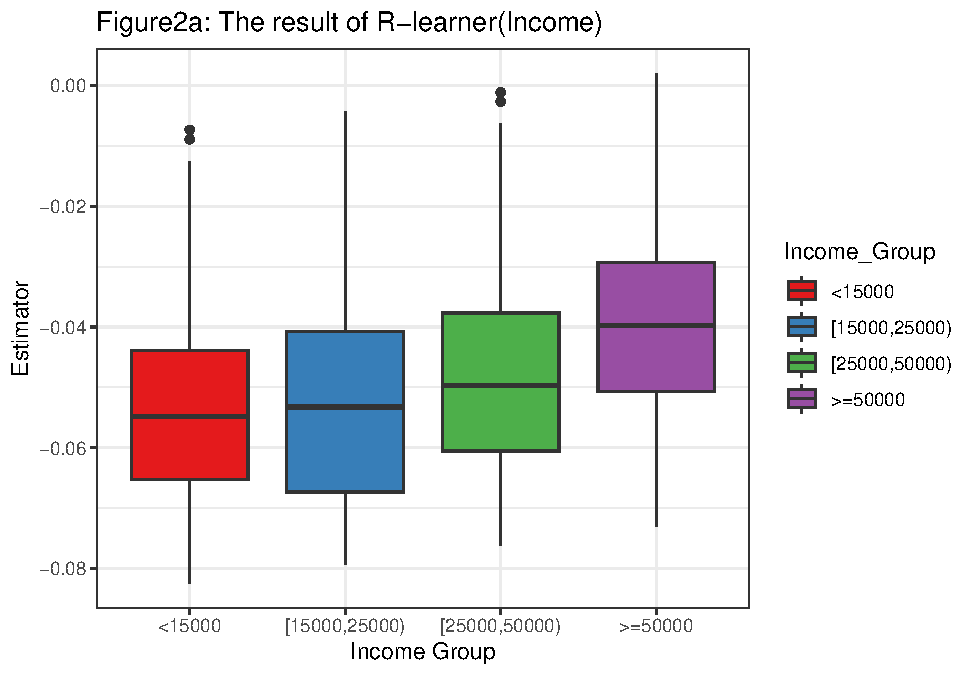
\includegraphics{template_files/figure-latex/unnamed-chunk-5-1.pdf}
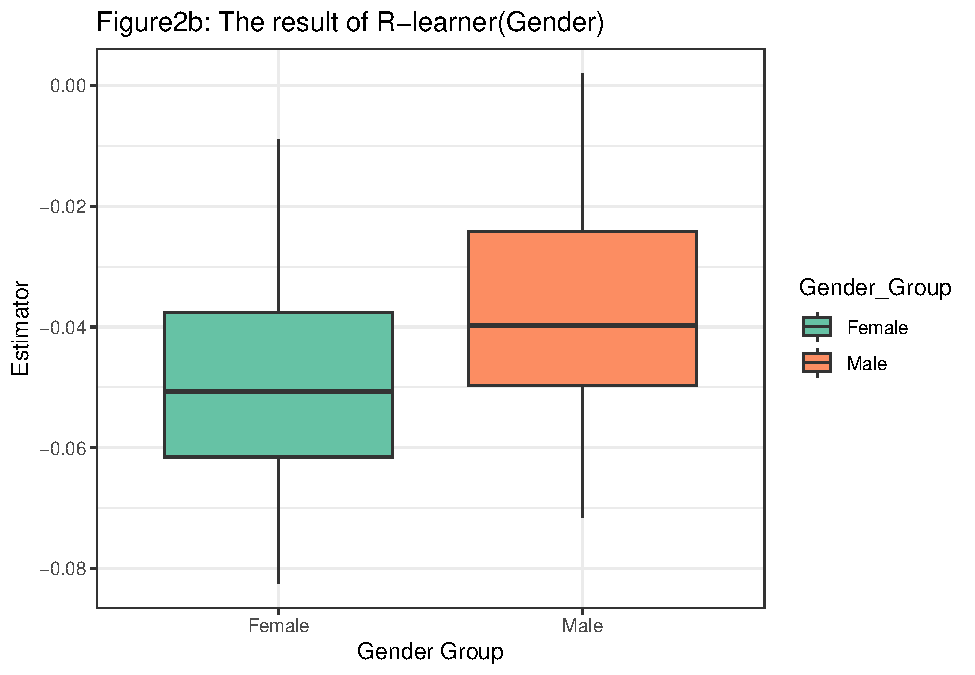
\includegraphics{template_files/figure-latex/unnamed-chunk-5-2.pdf}
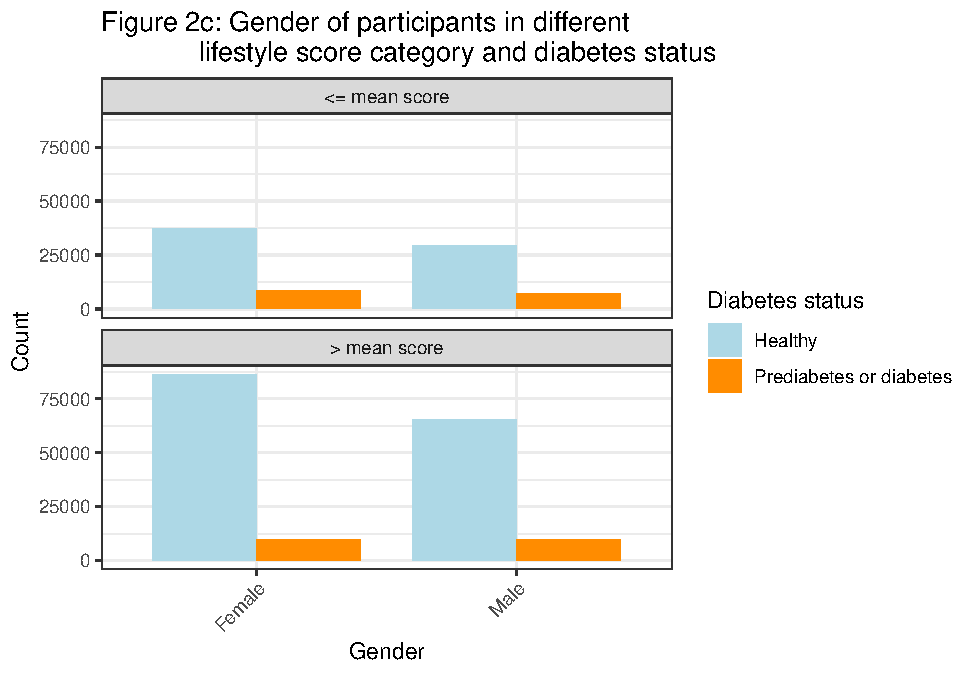
\includegraphics{template_files/figure-latex/unnamed-chunk-5-3.pdf}

\begin{longtable}[]{@{}lccc@{}}
\caption{Adjustment Results}\tabularnewline
\toprule()
& Estimate & 2.5 \% & 97.5 \% \\
\midrule()
\endfirsthead
\toprule()
& Estimate & 2.5 \% & 97.5 \% \\
\midrule()
\endhead
score & 0.5499 & 0.5374 & 0.5626 \\
adjusted score & 0.6856 & 0.6692 & 0.7024 \\
\bottomrule()
\end{longtable}

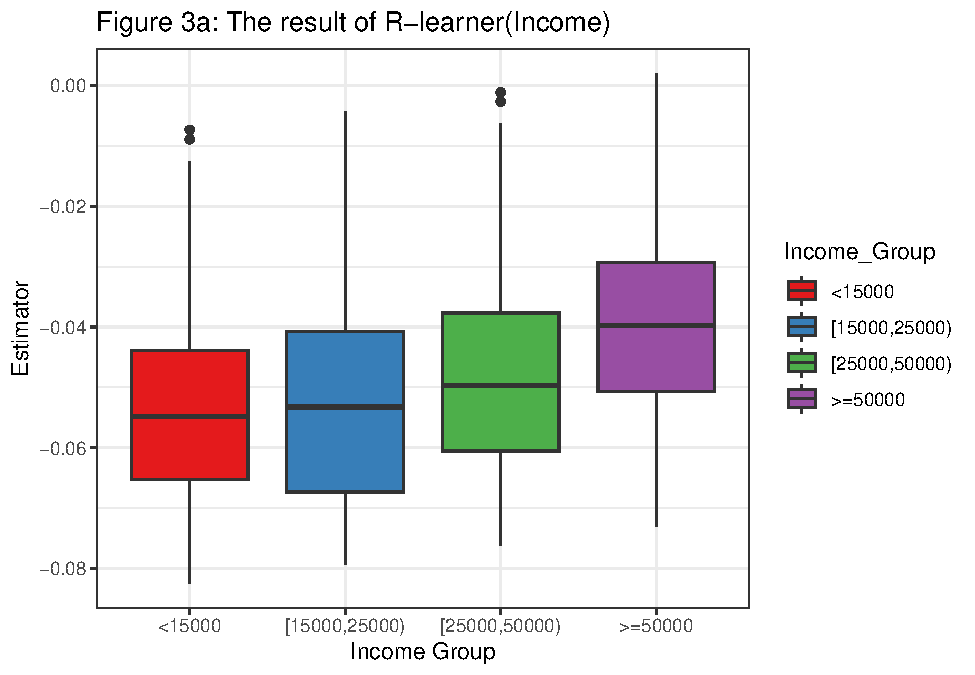
\includegraphics{template_files/figure-latex/unnamed-chunk-8-1.pdf}
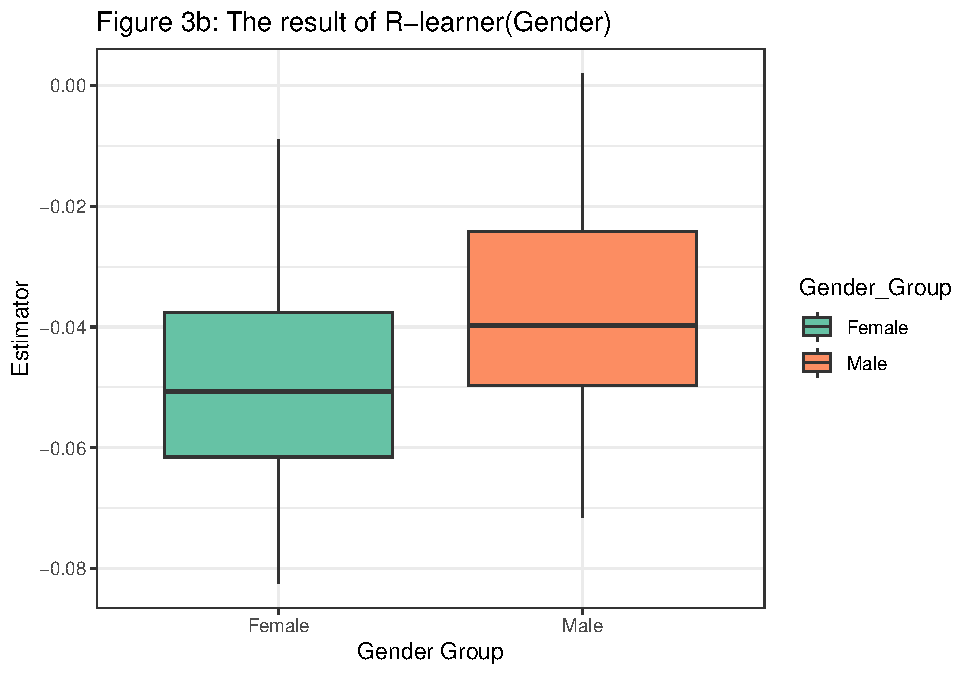
\includegraphics{template_files/figure-latex/unnamed-chunk-8-2.pdf}
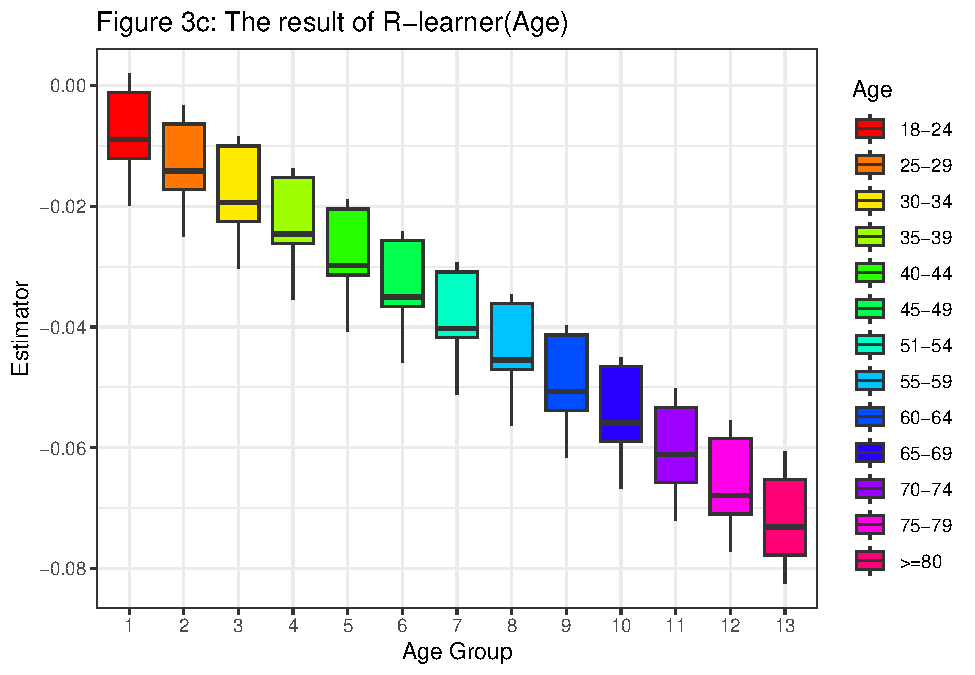
\includegraphics{template_files/figure-latex/unnamed-chunk-8-3.pdf}

\hypertarget{discussion}{%
\subsection{Discussion}\label{discussion}}

\hypertarget{target-trial}{%
\subsubsection{Target trial}\label{target-trial}}

The key causal question we try to answer in this analysis is ``whether
lifestyle is a risk factor for developing prediabetes or diabetes in
healthy participants''. Some basic criteria are expected to be satisfied
in order to build causality between the exposure and outcome of
interest, such as: (1) strength of association, (2) temporality, (3)
consistency, (4) dose-response relationship, (5) biologically or
theoretically plausible, (6) coherence, (7) specificity, and (8)
consensus among experts and the scientific community. The data of this
analysis derives from the cross sectional questionnaire of BRFSS program
in 2015, which has undermined the ability to build temporality between
lifestyles and the development of prediabetes and diabetes. In an ideal
situation to answer this causal question, a randomized controlled
experiment should be conducted, where healthy participants are assigned
to two groups of interventions and remain for a certain period of time,
such as 3 years. One group of people are required to adopt healthy
lifestyle including all the requirements mentioned below: ``lifetime
smoking less than 100 cigarettes'', ``doing physical activity or
exercising during the past 30 days other than their regular job'',
``consume fruit 1 or more times per day'', ``consume vegetables 1 or
more times per day'', and ``never drinking more than 14 drinks and 7
drinks per week for adult men and adult women, respectively''. Another
group of people are required to adopt an unhealthy lifestyle, which is a
reverse of the requirements in the healthy lifestyle group. All the
participants are expected to adhere to their assigned interventions
during the whole research period. However in reality, such a randomized
trial is inapplicable not only due to ethical constraints, but also due
to the limitations of precise definition of ``healthy lifestyle'' as
well as the difficulties to let participants adhere strictly to the
assigned lifestyles in everyday life.

In our analysis, a weighted combination score was created by integrating
participants' physical activity, smoking history, and alcohol, fruits,
and vegetable consumption. Then based on the combination score,
participants were grouped as ``having the score higher than the mean
score of all the participants'' or ``less than or equal to the mean
score of all the participants''. We take these categories as a
proximation of the interventions that participants may receive in an
RCT. However, people in the ``higher than mean score'' group does not
necessarily mean they satisfy all the five requirements for a healthy
lifestyle intervention in a RCT. We assume participants with higher than
the mean score would in general adopt healthier lifestyles in our
analysis. And thus, although we try to approach the true causal effect
using this observational study, the effect between lifestyle factors and
the risk of developing prediabetes or diabetes that we inferred from
this observational study is different from the inference from an RCT.

\hypertarget{refined-management-of-diabetes}{%
\subsubsection{Refined Management of
Diabetes}\label{refined-management-of-diabetes}}

Based on the estimated heterogeneity in treatment effects among
subgroups (defined by factors age, income, and gender), it is clear that
different groups respond differently to the treatment. Therefore, we can
identify susceptible groups for prioritized preventive measures.

From the perspective of income, it is crucial to pay particular
attention to the low-income population. If their lifestyle is subpar and
they lack the means to improve their current health status, the impact
of their lifestyle becomes even more significant. Looking at it from an
age standpoint, middle-aged and elderly individuals inherently have
slower metabolic rates compared to younger people. If they continue to
maintain unhealthy habits, they are more likely to develop illnesses. In
terms of gender, poor lifestyle habits have a greater effect on women.
Therefore, it is especially important for women, more so than men, to
establish healthy lifestyle habits.

\hypertarget{conclusion}{%
\subsection{Conclusion}\label{conclusion}}

\begin{itemize}
\tightlist
\item
  Healthier lifestyle is associated with lower risk of developing
  prediabetes or diabetes;
\item
  Limitations exist in cross-sectional studies in inferring causal
  inference between independent variables and dependent variables;
\item
  We can identify vulnerable groups for prioritized preventive measures
  based on the heterogeneous treatment effect. We need to pay particular
  attention to the low-income population, women, and middle-aged to
  elderly individuals.
\end{itemize}

\hypertarget{references}{%
\subsection{References}\label{references}}

Lin, X., Xu, Y., Pan, X., Xu, J., Ding, Y., Sun, X., . . . Shan, P. F.
(2020). Global, regional, and national burden and trend of diabetes in
195 countries and territories: an analysis from 1990 to 2025. Sci Rep,
10(1), 14790. \url{doi:10.1038/s41598-020-71908-9}

Centers for Disease Control and Prevention. (n.d.). Behavioral Risk
Factor Surveillance System. Retrieved May 4, 2023, from
\url{https://www.cdc.gov/brfss/index.html}

Centers for Disease Control and Prevention (CDC). Behavioral Risk Factor
Surveillance System Survey Data. Atlanta, Georgia: U.S. Department of
Health and Human Services, Centers for Disease Control and Prevention,
2015.

Bird, Y., Lemstra, M., Rogers, M., \& Moraros, J. (2015). The
relationship between socioeconomic status/income and prevalence of
diabetes and associated conditions: A cross-sectional population-based
study in Saskatchewan, Canada. International journal for equity in
health, 14, 93. \url{https://doi.org/10.1186/s12939-015-0237-0}

Nanayakkara N, Curtis AJ, Heritier S, et al.~Impact of age at type 2
diabetes mellitus diagnosis on mortality and vascular complications:
systematic review and meta-analyses. Diabetologia. 2021;64(2):275--287.
\url{doi:10.1007/s00125-020-05319-w}

Cinelli, C., Forney, A., \& Pearl, J. (2022). A Crash Course in Good and
Bad Controls. Sociological Methods \& Research, 0(0).
\url{https://doi.org/10.1177/00491241221099552}

Ali O. (2013). Genetics of type 2 diabetes. World journal of diabetes,
4(4), 114--123. \url{https://doi.org/10.4239/wjd.v4.i4.114}

Spirtes, P., Glymour, C., \& Scheines, R. (2012) Causation, Prediction,
and Search. MIT Press.

Nie, X., Wager, S. (2021). Quasi-oracle estimation of heterogeneous
treatment effects, Biometrika, 108(2), 299--319.
\url{https://doi.org/10.1093/biomet/asaa076}

Schofield, J. D., Liu, Y., Rao-Balakrishna, P., Malik, R. A., \& Soran,
H. (2016). Diabetes Dyslipidemia. Diabetes therapy : research, treatment
and education of diabetes and related disorders, 7(2), 203--219.
\url{https://doi.org/10.1007/s13300-016-0167-x}

Petrie, J. R., Guzik, T. J., \& Touyz, R. M. (2018). Diabetes,
Hypertension, and Cardiovascular Disease: Clinical Insights and Vascular
Mechanisms. The Canadian journal of cardiology, 34(5), 575--584.
\url{https://doi.org/10.1016/j.cjca.2017.12.005}

\newpage

\hypertarget{appendix}{%
\subsection{Appendix}\label{appendix}}

\hypertarget{definition-adjustment-criterion-shpitser-et-al.-2012}{%
\subsubsection{Definition (adjustment criterion (Shpitser et al.,
2012))}\label{definition-adjustment-criterion-shpitser-et-al.-2012}}

A set of variables Z in the adjustment set satisfies the adjustment
criterion relative to (X, Y) in a DAG G if:

\begin{itemize}
\tightlist
\item
  No element in Z is a descendant in \(G_{\Bar{x}}\) (the DAG G without
  the edges with arrows coming into X) of any \(W \notin X\) which lies
  on a proper causal path from X to Y.
\item
  All non-causal paths in G from X to Y are blocked by Z.
\end{itemize}

\hypertarget{dag}{%
\subsubsection{DAG}\label{dag}}

\end{document}
